\documentclass[12pt]{article}

\input preamble

\title{Principles of Parallel Architecture\\
Homework 2: Parallel Programming Models}
\author{Xitong Liu \\
xliu@ece.udel.edu}

\begin{document}

\maketitle

\section{MPI Program development}
\begin{enumerate}

\item Ring program
\begin{description}
\item[Q:] The MPI ring program is one of the simplest programs 
that can be written in MPI. The intention of a MPI ring 
program is to write, in order, numbers from 1 to p, where 
p is the total number of processes being used. As a further 
restriction, each process can only write a single, unique 
number in the following way:
\begin{verbatim}
Process number 1 writes number 1
Process number 2 writes number 2
...
Process number p writes number p
\end{verbatim}
\item[A:]  The source code can be located both in \texttt{ring1} 
and \texttt{ring2} directories, with \texttt{Makefile} provided.
Type \texttt{make run} to compile and run the program with results
generated.
\end{description}

\item
\begin{description}
\item[Q:] The parallel sum program: The objective of this 
program is to obtain the summation of 1000 numbers using 
N processors. To do so, at the beginning the numbers are 
distributed among the available processes.
\end{description}
\item[A:] The source code can be located in \texttt{mpi\_parallel\_sum}.
Type \texttt{make run} to compile and run the program with results
generated.
\end{enumerate}

\section{OpenMP program development}
\begin{enumerate}

\item Parallel hello world program
\begin{description}
\item[Q:] This program will print �Hello world from thread i of p� 
where i is the thread number and p is the total number of threads. 
The number of threads to be used should be a parameter that is 
passed through the command line.
\item[A:] The source code can be located in \texttt{omp\_hello\_world}.
Type \texttt{make run} to compile and run the program with results
generated.
\end{description}

\item The parallel sum program
\begin{description}
\item[Q:] The program�s intention is the same as before. The number 
of threads to be used should be a parameter that is passed through 
the command line.

However, the partition is not done by the programmer; instead, use 
the parallel for clause of openmp to distribute numbers to threads 
and to initialize the random numbers.

Use a private variable to accumulate the result in the loop and 
then use atomic operations to produce the final sum.

Measure the running time of the parallel computation and make a 
graph time vs number of threads. Comment about the results.

\item[A:] The source code can be located in \texttt{omp\_parallel\_sum}.
Type \texttt{make run} to compile and run the program with results
generated.
\begin{figure}[h!]
	\begin{center}
		\includegraphics[width=1.0\textwidth, angle=0]{omp_sum.pdf}
		\caption{\label{fig:omp_sum}OpemMP Sum time vs number of threads}
	\end{center}
\end{figure}
\end{description}
\end{enumerate}

\section{Pthread program development}
\begin{enumerate}

\item The parallel hello world program
\begin{description}
\item[Q:] Achieve the same results obtained using OpenMP, but this time
use pthreads.
\item[A:] The source code can be located in \texttt{pthread\_hello\_world}.
Type \texttt{make run} to compile and run the program with results
generated.
\end{description}

\item The parallel sum program
\begin{description}
\item[Q:] The objective is the same as the previous parallel sum programs. 
However, thread synchronization is not explicit in pthread programming.

Measure the running time of the parallel computation and make a graph 
time vs number of threads. Comment about the results.
\item[A:] The source code can be located in \texttt{pthread\_parallel\_sum}.
Type \texttt{make run} to compile and run the program with results
generated.
\begin{figure}[h!]
	\begin{center}
		\includegraphics[width=1.0\textwidth, angle=0]{pthread_sum.pdf}
		\caption{\label{fig:pthread_sum}Pthread Sum time vs number of threads}
	\end{center}
\end{figure}
\end{description}
\end{enumerate}

\section{Cilk programming}
\begin{enumerate}

\item The Head-Tails game
\begin{description}
\item[Q:] In the head-tails game, a player throws a coin 5 times and 
then he counts the number of times that he obtained heads. If the player 
obtained heads at least 3 times, he wins, otherwise he loses.
\item[A:] The source code can be located in \texttt{cilk\_coin\_game}.
Type \texttt{make run} to compile and run the program with results
generated.
\end{description}

\end{enumerate}

\end{document}

\begin{comment}
\begin{figure}[h!]
	\begin{center}
		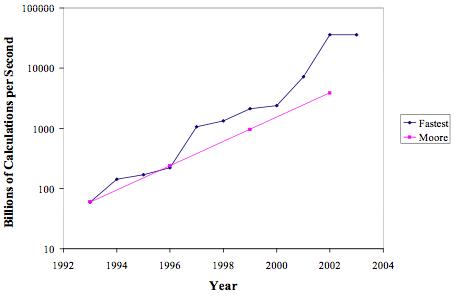
\includegraphics[width=0.7\textwidth, angle=0]{fatest.png}
		\caption{\label{fig:fatest}Fatest SuperComputer in the world}
	\end{center}
\end{figure}
\end{comment}